\documentclass[10pt,a4paper]{article}
\usepackage[utf8]{inputenc}
\usepackage[french]{babel}
\usepackage[T1]{fontenc}
\usepackage{amsmath}
\usepackage{amsfonts}
\usepackage{amssymb}
\usepackage{graphicx}
\usepackage[lofdepth,lotdepth]{subfig}
\usepackage[left=2cm,right=2cm,top=2cm,bottom=2cm]{geometry}
\usepackage{physics} %Physics.sty
\author{Loann Brahimi}
\title{Détermination du taux de turbulence des ondes de Alfvén par équilibre du taux de croissance et d'amortissement des ondes de Alfvén dans les milieux faiblement ionisés}
\begin{document}
\maketitle 

\section*{Coefficients d'amortissement par collisions ions-neutres}

Dans ce document nous allons calculer le coefficient d'amortissement des ondes de Alfvén par collisions des ions avec les neutres dans le cadre d'un milieu faiblement ionisé. On écrit dans un premier temps la relation de dispersion des ondes de Alfvén incluant un amortissement suivant les collisions neutre-ion et la viscosité des neutres. On a (Xu 2015) :

\begin{equation}
	\omega^3 + i\left({\tau_v}^{-1} + (1+\chi)\nu_{ni}\right)\omega^2 - \left(k^2\cos^2{\theta} {V_{Ai}}^2 + 
	\chi{\tau_v}^{-1}\nu_{ni}\right)\omega - i\left({\tau_v}^{-1} + \nu_{ni}\right)k^2\cos^2{\theta} {V_{Ai}}^2 = 0
	\label{1}
\end{equation}

où $\chi = \rho_n / \rho_i$ et ${\tau_v}^{-1} = k^2 \nu^n$. Dans un premier temps, on néglige la viscosité cinématique des neutres $\nu_n \approx 0$, l'équation \ref{1} devient : 

\begin{equation}
	\omega^3 + i(1+\chi)\nu_{ni}\omega^2 - k^2\cos^2{\theta} {V_{Ai}}^2\omega - i\nu_{ni}k^2\cos^2{\theta} {V_{Ai}}^2 = 0
	\label{2}
\end{equation}

Xu+2015 propose des solutions analytiques dans le cas d'un amortissement faible c'est à dire $\abs{\Gamma_{in}} \ll \abs{\omega_R}$. 

\begin{eqnarray}
	{\omega_R}^2 & = & \frac{k^2\cos^2{\theta}{V_{Ai}}^2 \left[(1+\chi){\nu_{ni}}^2 + k^2 \cos^2{\theta} {V_{Ai}}^2\right]}{(1+\chi)^2{\nu_{ni}}^2 + k^2 \cos^2{\theta} {V_{Ai}}^2} \\
	\Gamma_{in}  & = & - \frac{\nu_{ni}\chi  k^2 \cos^2{\theta} {V_{Ai}}^2}{2\left[ (1+\chi)^2{\nu_{ni}}^2 + k^2 \cos^2{\theta} {V_{Ai}}^2 \right]}
\end{eqnarray}

Dans le cas d'un couplage fort ($\omega \ll \nu_{in}$) on a : 

\begin{eqnarray}
	{\omega_{R,s}}^2 & = & {V_{A}}^2 k^2 \cos^2{\theta} \\ 
	\Gamma_{in,s}  & = & - \frac{\xi_n  {V_{A}}^2 k^2 \cos^2{\theta}}{2 \nu_{ni}}
\end{eqnarray}


Dans le cas d'un couplage faible ($\omega \gg \nu_{in}$) on a : 

\begin{eqnarray}
	{\omega_{R,w}}^2 & = & {V_{Ai}}^2 k^2 \cos^2{\theta} \\ 
	\Gamma_{in,w}  & = & - \frac{\nu_{in}}{2} \label{taux_fort}
\end{eqnarray}

avec $\nu_{in} = \frac{m_n}{m_i + m_n}n_n \expval{\sigma v}$ et $\nu_{ni} = \frac{m_i}{m_i + m_n}n_i \expval{\sigma v}$ (Kulsrud et al. 1971 propose une évaluation du terme $\expval{\sigma v}$ en fonction de la température, Jean et al. 2009 propose une formulation empirique, la dernière option est utilisée dans le présent calcul). Dans toute la suite, on considère des modes slab c'est à dire de vecteur d'onde le long des lignes de champ non-perturbées, ceci impliquant la condition $\cos{\theta} = 1$. \\ 

Pour chacun des régimes on peut déterminer une échelle de coupure des ondes de Alfvén caractérisée par $\abs{\Gamma_{in}} \approx \abs{\omega_R}$. Dans l'intervalle $[k^+_c, k^-_c]$ où $k^+_c = 2\nu_{ni}/(V_A \xi_n)$ et $k^-_c = \nu_{in}/(2V_{Ai})$, les ondes de Alfvén ne se propagent pas. A toutes les échelles plus grandes que $k^+_c$ les ions et les neutres sont fortement couplés impliquant ainsi un faible amortissement des ondes de Alfvén tandis qu'à toutes les échelles plus petites que $k^-_c$ les ions et les neutres sont faiblement couplés impliquant un fort amortissement des ondes de Alfvén. 

\section*{Détermination du taux de turbulence}

On peut également, en suivant la méthode utilisée par Wiener + 2013, déterminer le taux de turbulence $b_k = \delta B / B$ à partir de la condition d'équilibre des ondes de Alfvén entre taux de croissance et taux d'amortissement par collision ions-neutres. Les formules (26) et (25) de Wiener + 2013 donnent : 

\begin{equation}
	\Gamma_{\mathrm{growth}}(k) = - \frac{2\pi m \Omega_0 V_A c}{k B_0^2}\left(\frac{B}{\delta B}\right)^2 \pdv{n_{CR}}{z} A(k)
\end{equation}

où $\delta B / B = b_k$ est le niveau de turbulence et d'après (24) de Wiener + 2013 :

\begin{equation}
A(k) = \frac{1}{n_{CR}} \int^\infty_{p_k} \dd p \beta f(p) 4\pi (p^2 - p_k^2) ~~~ 0 \leq A(k) \leq 1
\end{equation}

En posant $\Gamma_\mathrm{growth} + \Gamma_{in} = 0$, il est possible de contraindre $b_k$ suivant le milieu considéré. En définissant $r_g = k^{-1}$, $k$ étant le nombre d'onde des perturbations produites par un RC de rayon de gyration $r_g$, n trouve : 

\begin{equation}
	b_k(r_g) = \sqrt{\frac{1}{-\Gamma^i_{in,s/w}} \frac{3}{4} \Omega_0 \left(V_{A(i)} \frac{mc}{p_0c} \right) A(r_g) \frac{H}{G} \left( \frac{r_g}{W_B}  \left[ - \pdv{P_{CR}}{z} \right] \right)}
\end{equation}

avec les relations : 


\begin{eqnarray}
	f(p) & = & f_0 k(p) \\ 
	A(k)    & = & \frac{4\pi}{n_{CR}} f_0 p_0^3 \int^{+\infty}_{\mathrm{max}(p_k/p_c, 1)} \dd \bar{p} \beta(\bar{p}) k(\bar{p}) (\bar{p}^2 - \bar{p}^2_k)  \\ 
	H & = & \int^{+\infty}_{p_c/p_0} \dd\bar{p} ~ \bar{p}^2 k(\bar{p}) \\ 
	G & = & \int^{+\infty}_{p_c/p_0} \dd \bar{p}~\bar{p}^3 k(\bar{p}) \beta(\bar{p}) \\
	\beta(\bar{p}) & = & \frac{\bar{p}}{\sqrt{\bar{p}^2 + 1}} \\
	n_{CR} & = & 4\pi f_0 p_0^3 H \\ 
	P_{CR} & = & \frac{4 \pi c}{3} f_0 p_0^4 G \\ 
\end{eqnarray}

où $p_c$ est le moment de coupure de la fonction de distribution des RCs.
Il s'agit maintenant de choisir la forme de la fonction de distribution des rayons cosmiques adaptée au problème. Drury et Strong 2016 ont choisi une fonction de la forme : 

\begin{equation}
	J(T) = 0.27(\mathrm{cm}^{-2}~\mathrm{s}^{-1}~\mathrm{st}^{-1}~\mathrm{GeV}^{-1})\frac{T^{1.12}}{\beta^2} \left( \frac{T+0.67}{1.67} \right)^{-3.93}
\end{equation}

où $T = E_{kin}/1~\mathrm{GeV}$ soit $T = \frac{mc^2}{1~\mathrm{GeV}} (\sqrt{1 + (p/p_0)^2}-1)$ et $\dv{T}{p} = \frac{mc^2}{p_0} \frac{p/p_0}{\sqrt{1 + (p/p_0)^2 }}$. On rappelle que l'on a défini $p_0c = mc^2$. On peut alors réécrire la fonction $f(p)$ comme :

\begin{equation}
	f(\bar{p}) = f_0 k(\bar{p})~~ f_0 = \frac{0.27}{p_0^2}
\end{equation}

\begin{equation}
	k(\bar{p}) = \frac{1}{\bar{p}^2} \frac{({mc^2}_{1~\mathrm{GeV}}[\sqrt{1+\bar{p}^2} - 1])^{1.12}}{\beta^2(\bar{p})} \left( \frac{{mc^2}_{1~\mathrm{GeV}}[\sqrt{1+\bar{p}^2} - 1] + 0.67}{1.67} \right)^{-3.93} 
\end{equation}

où ${mc^2}_{1~\mathrm{GeV}}$ correspond à l'énergie de masse des CRs normalisée par $1~\mathrm{GeV}$. \\ 

\begin{figure}
	\centering
	\includegraphics[width=0.5\textwidth]{./figures/distribution_function.eps}
	\label{dist_func}
	\caption{Fonction de distribution des rayons cosmiques}
\end{figure}


\section*{Application aux milieux astrophysiques faiblement ionisés}

Nous déterminons dans cette partie le niveau de turbulence de Alfvén dans les phases WNM, CNM, DiM, DeM et DeC de l'ISM dont les paramètres physiques sont précisés dans la figure \ref{fig:results}. On considère également une densité caractéristique de RCs donnée par $n_0 = 0.27/c~\mathrm{cm}^{-3}\mathrm{st}^{-1}\mathrm{GeV}^{-1}$ (Drury et Strong 2016) et un gradient caractéristique moyen de pression de RCs donné par $\pdv{P_{CR}}{z} = 10^{-29}~\mathrm{erg}~\mathrm{cm}^{-4}$ (Wiener et al. 2013). \\ 


Dans la phase WNM (figure \ref{sub:WNM}), en régime de fort amortissement nous observons que le taux de turbulence croit en $\bar{T}^{0.24}$ jusqu'à $T/mc^2 \approx 0.2$ puis décroît en $\bar{T}^{-0.36}$ jusqu'à la bande de coupure des ondes de Alfvén $\bar{T} \in [1.4\times 10^{2}, 1.7\times 10^{3}]$. Ceci est principalement dû à la distribution en énergie des CRs dont l'impulsion de coupure est donnée par $p_c = 10^{-2}p_0$. En régime de faible amortissement, le taux de turbulence se met à re-croitre en $\bar{T}^0.59$. Ce changement de comportement est dû à la dépendance en $k^2$ du taux d'amortissement par collisions ions-neutres. \\ 

Dans la phase CNM (figure \ref{sub:CNM}), en régime de fort amortissement nous observons que le taux de turbulence croit avec le même indice et jusqu'au même maximum que pour la phase WNM à la différence que la bande interdite est décalée vers les énergies plus faibles et est élargie ($\bar{T} \in [5.5\times 10^{-1}, 1.6\times 10^{1}]$). En régime de faible amortissement, le taux de turbulence remonte avec la même pente que pour la phase WNM. L'élargissement de la bande de coupure est principalement dû à l'augmentation du rapport $\rho_n / \rho_i$ et son décalage vers les faibles énergies est dû à la diminution de la vitesse de Alfvén et de la température cinétique. \\ 

Pour les milieux moléculaires (figures \ref{sub:DiM}, \ref{sub:DeM} et \ref{sub:DeC}), la bande interdite est de plus en plus large à mesure que la densité du milieu augmente et est de plus en plus décalée vers les basses énergies. Cela signifie que dans les milieux moléculaires, les ondes de Alfvén sont très facilement amorties à faible énergie. 


 
\begin{figure}[t!]
  \begin{center}
    \subfloat[WNM - $E_c = 10~\mathrm{MeV}$]{
      \includegraphics[width=0.5\textwidth]{./figures/WNM.eps}
      \label{sub:WNM}
                         }
    \subfloat[CNM - $E_c = 10~\mathrm{MeV}$]{
      \includegraphics[width=0.5\textwidth]{./figures/CNM.eps}
      \label{sub:CNM}
                         } \\
    \subfloat[DiM - $E_c = 10~\mathrm{MeV}$]{
      \includegraphics[width=0.5\textwidth]{./figures/DiM.eps}
      \label{sub:DiM}
                         } 
    \subfloat[DeM - $E_c = 10~\mathrm{MeV}$]{
      \includegraphics[width=0.5\textwidth]{./figures/DeM.eps}
      \label{sub:DeM}
                         }  \\ 
    \subfloat[DeC - $E_c = 10~\mathrm{MeV}$]{
      \includegraphics[width=0.5\textwidth]{./figures/DeC.eps}
      \label{sub:DeC}
                         }             
    \caption{Les graphes ci-dessus représentent le comportement du taux de turbulence des ondes de Alfvén en fonction de l'énergie cinétique normalisée par l'énergie de masse des RCs. En (a) est représenté le taux de turbulence dans la phase WNM de paramètres : $T = 6\times 10^3~\mathrm{K}$, $B = 5\times 10^{-6}~\mathrm{G}$, $f_{ion} = 7\times 10^{-3}$ et $n_H = 0.2~\mathrm{cm}^{-3}$. En (b) est représenté le taux de turbulence dans la phase CNM de paramètres : $T = 50~\mathrm{K}$, $B = 6\times 10^{-6}~\mathrm{G}$, $f_{ion} = 4\times 10^{-4}$ et $n_H = 20~\mathrm{cm}^{-3}$. En (c) est représenté le taux de turbulence dans la phase DiM de paramètres : $T = 30~\mathrm{K}$, $B = 4.9\times 10^{-6}~\mathrm{G}$, $f_{ion} = 5\times 10^{-4}$ et $n_H = 100~\mathrm{cm}^{-3}$. En (d) est représenté le taux de turbulence dans la phase DeM de paramètres : $T = 10~\mathrm{K}$, $B = 14\times 10^{-6}~\mathrm{G}$, $f_{ion} = 1\times 10^{-4}$ et $n_H = 500~\mathrm{cm}^{-3}$. En (e) est représenté le taux de turbulence dans la phase DeC de paramètres : $T = 10~\mathrm{K}$, $B = 22\times 10^{-6}~\mathrm{G}$, $f_{ion} = 1\times 10^{-6}$ et $n_H = 1000~\mathrm{cm}^{-3}$. La majorité des données sont issues de Jean et al. 2009.}
    \label{fig:results}
  \end{center}
\end{figure}



\section*{Détermination du libre parcours moyen des RCs dans la phase WIM dominé par l'amortissement ion-neutre} 

Dans cette partie, nous cherchons à déterminer le libre parcours moyen des RCs dans une phase tiède dont le taux d'ionisation est élevé en supposant que les ondes de Alfvén sont principalement amorties par les collisions ions-neutres. On considère trois taux d'amortissement (de croissance) des ondes de Alfvén : 

\begin{eqnarray}
	\Gamma_\mathrm{growth} & = & \frac{3}{4}\Omega_0 \left(V_A \frac{mc}{p_0c} \right) \frac{A(r_g)}{b_k^2} \frac{H}{G} \left[\frac{r_g}{W_{B_0}} \left(-\pdv{P_{CR}}{z}\right) \right] \\ 
	\Gamma_{in} & = & - \nu_{in}/2  \\ 
	\Gamma_{NLLD} & = & - \sqrt{\frac{\pi}{8}} v_i k b_k^2 
\end{eqnarray}

$\Gamma_\mathrm{growth}$ est le taux de croissance des ondes de Alfvén que nous avons précédemment calculé. $\Gamma_{in}$ est de taux d'amortissement des ondes de Alfvén par collisions ions-neutres en régime faiblement couplé. En effet, la phase WIM est fortement ionisée impliquant que l'abondance de neutres est très faible ce qui permet de choisir l'expression du coefficient d'amortissement ion-neutre en régime faiblement couplé dont l'expression est plus simple. Enfin $\Gamma_{NLLD}$ est l'amortissement de Landau non-linéaire qui résulte du transfert d'énergie des ondes de Alfvén vers les RCs. Ce denier dépend du taux de turbulence et de la vitesse thermique (parallèle) des ions donnée par $v_i = \sqrt{k_B T / m_i}$. \\ 

On détermine dans un premier temps le niveau de turbulence en égalisant les différents taux, on trouve : 

\begin{equation}
	b_k^2 = \sqrt{\frac{2}{\pi}} \frac{\nu_{in}r_g}{2v_i} \left[ -1 + \sqrt{1+R} \right]
\end{equation}

où $R = 6 \sqrt{\frac{\pi}{2}} \frac{\Omega_0 v_i}{\nu_{in}^2} \left( V_A \frac{mc}{p_0 c} \right) \frac{H}{G} \left[W_{B_0}^{-1} \left( - \pdv{P_{CR}}{z} \right) \right] A(r_g)$. Lorsque l'amortissement ions-neutres domine ($\nu_{in} \gg 1$), $R \ll 1$ et le taux de turbulence s'écrit : $b_k^2 = \sqrt{\frac{2}{\pi}} \frac{\nu_{in}r_g}{2v_i} R$. En utilisant la définition du libre parcours moyen des RCs de Wiener 2013 : $\lambda = v_i/\nu$ où $\nu= \frac{\pi}{4}\Omega_0 b_k^2$ on trouve : 

\begin{equation}
	\lambda = \sqrt{\frac{8}{\pi}} \frac{4 v_i}{\nu_in} R^{-1}
\end{equation}

Les résultats (figure \ref{libre_parcours}) concordent avec ceux de Wiener 2013 confirmant ainsi la validité des calculs du taux de croissance des ondes de Alfvén et le taux de turbulence déterminé pour les phases partiellement ionisées de l'ISM. 
\begin{figure}
\centering
	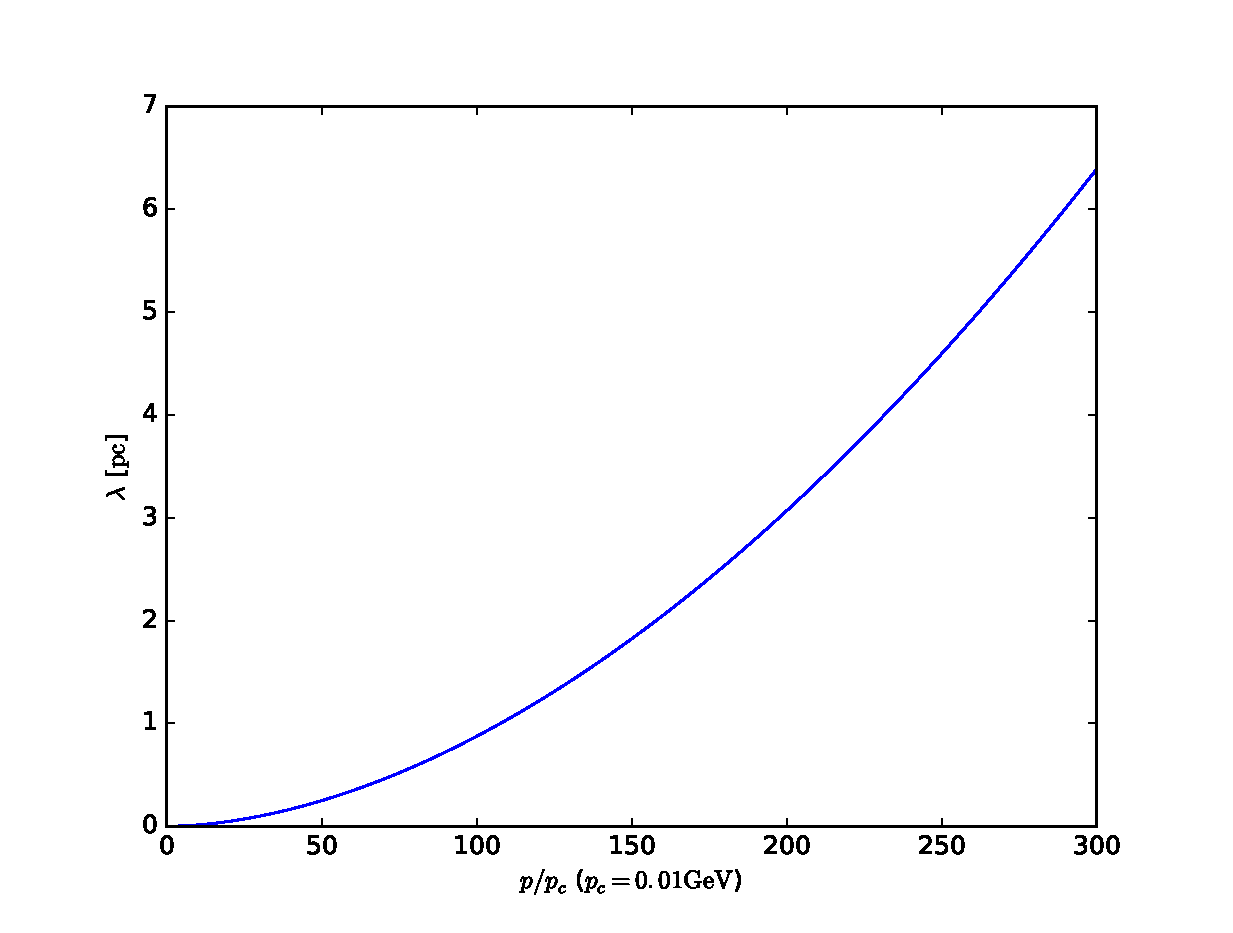
\includegraphics[scale=0.5]{./figures/libre_parcours_moyen.eps}
\label{libre_parcours}
\caption{Libre parcours moyen des RCs obtenu dans l'approximation de fort amortissement des ondes de Alfvén par collision ions-neutres dans la phase WIM de paramètres suivants : $T= 1\times 10^{4}~\mathrm{K}$, $B=5~\mu\mathrm{G}$, $n_H = 0.0125~\mathrm{cm}^{-3}$, $f_{ion} = 0.8$, Gradient moyen = $1\times 10^{-34}~\mathrm{erg}~\mathrm{cm}^{-4}$.}
\end{figure}













%%%%%%%%%%%%%%%%%%%%%%%%%%%%%%%%%%%%%%%%%%%%%%%%%%%%%%%%%%%%%%%%%%%%%%%%%%%%%%%%%%%%%%%%%%%%%%%%%%%%%%%%%%%%%
\appendix

\section{Récapitulatif des différents paramètres numériques du calcul}
\label{para_num}

\begin{center}
\begin{tabular}{|c|}
\hline
WNM \\
\hline
\hline  
\bf{Abondances et taux d'ionisation}\\ 
\hline
$T = 6000 - 10~000~\mathrm{K}$ et $B \approx 5 \mu\mathrm{G}$ \\  
Abondances : $n_{He}/n_H \approx 0.07$ \\ 
Neutre dominant : $H+0.07H_e$ $m_n \approx m_p + 0.07\times 4 m_p = 2.14 \times 10^{-24}~\mathrm{g}$ \\ 
Ion dominant : $H^+$ $m_{H^+} = m_p = 1.67 \times 10^{-24}~\mathrm{g}$    \\
\hline
$n_H = 0.2 - 0.5~\mathrm{cm}^3$ et $f_\mathrm{ion} = \frac{n_i}{n_i+n_n} = 0.007-0.05$ \\ 
$n_n = 1.07\times (1-f_\mathrm{ion})n_H = 0.20-0.52~\mathrm{cm}^{-3}$ et $n_i = 1.07\times f_\mathrm{ion}n_H = 0.0015 - 0.027~\mathrm{cm}^{-3}$ \\
$\xi_n = \frac{\rho_n}{\rho_n+\rho_i} = 0.88 - 0.99$ où $\rho_n = m_n n_n$ et $\rho_i = m_i n_i$ \\ 
\hline
\hline
\bf{Fréquences de collision et vitesses de Alfvén}\\
\hline
$\nu_{ni} \sim (1.4\times 10^{-9}~\mathrm{cm}^3~\mathrm{s}^{-1}) \sqrt{\frac{T}{100~\mathrm{K}}}n_i = 1.75\times 10^{-11} - 3.13\times 10^{-10}~\mathrm{s}^{-1}$ \\ 
$\nu_{in} \sim (1.4\times 10^{-9}~\mathrm{cm}^3~\mathrm{s}^{-1}) \sqrt{\frac{T}{100~\mathrm{K}}}n_n = 2.37\times 10^{-9} - 6.21\times 10^{-9}~\mathrm{s}^{-1}$ \\ 
\hline 
$V_A = B/\sqrt{4\pi m_p (n_n +n_i)} = 1.51\times 10^6 - 2.49 \times 10^6 ~\mathrm{cm}~\mathrm{s}^{-1}$ \\ 
$V_{Ai} = B/\sqrt{4\pi m_p n_i} = 6.90\times 10^6 - 2.91\times 10^7~\mathrm{cm}~\mathrm{s}^{-1}$ \\ 
\hline 
\hline
\bf{Taux d'amortissement par collision ions-neutres} \\ 
\hline
$\Gamma^\mathrm{WNM}_{in,s} = - \left[ 3.22\times 10^{3} \left( \frac{k}{10^{-9}~\mathrm{cm}^{-1}} \right)^2 - 1.77\times 10^{5} \left( \frac{k}{10^{-9}~\mathrm{cm}^{-1}} \right)^2 \right]~\mathrm{s}^{-1}$ si $\omega \ll \nu_{in}$ \\ 
$\Gamma^\mathrm{WNM}_{in,w} = - \left[ 1.19\times 10^{-9} - 3.11 \times 10^{-9} \right]~\mathrm{s}^{-1}$ si $\omega \gg \nu_{in}$ \\
\hline
\hline
\bf{Coefficients $C_i$} \\
\hline
$C^\mathrm{WNM}_s = \sqrt{\frac{2\pi qV_A}{B} \frac{1}{\Gamma^\mathrm{WNM}_{in,s}}} = \frac{1}{k} [ 7.17 \times 10^{-11} - 6.83 \times 10^{-10} ]$ si $\omega \ll \nu_{in}$ \\ 
$C^\mathrm{WNM}_w = \sqrt{\frac{2\pi qV_{Ai}}{B} \frac{1}{\Gamma^\mathrm{WNM}_{in,w}}} = 9.97\times 10^5 - 1.98 \times 10^6$ si $\omega \ll \nu_{in}$ \\ 
\hline 
\hline
\bf{Intervalle de non-validité de l'approximation $\abs{\Gamma^\mathrm{WNM}_{in}} \ll \omega_R$} \\ 
\hline
$k_{\mathrm{dec},ni,\mathrm{slab}} = \nu_{ni}/V_A = 7.02\times 10^{-18} - 2.07 \times 10^{-16} ~ \mathrm{cm}^{-1}$ \\ 
$k_{\mathrm{dec},in,\mathrm{slab}} = \nu_{in}/V_{Ai} = 8.15\times 10^{-17} - 9.00 \times 10^{-16} ~ \mathrm{cm}^{-1}$ \\ 
$\left[{k^+_{c,\mathrm{slab}}}_\mathrm{min}, {k^-_{c,\mathrm{slab}}}_\mathrm{max} \right] = [1.40 \times 10^{-17}, 4.50\times 10^{-16}] ~ \mathrm{cm}^{-1}$ \\ 
\hline
\hline
\bf{Énergies de coupure de la fonction de distribution en loi de puissance} \\ 
\hline
$E_c = 100~\mathrm{MeV} \leftrightarrow k^{100~\mathrm{MeV}}_c = 1.5\times 10^{-11}~\mathrm{cm}^{-1}$ \\ 
$E_c = 1~\mathrm{GeV} \leftrightarrow k^{1~\mathrm{GeV}}_c = 1.5\times 10^{-12}~\mathrm{cm}^{-1}$     \\ 
$E_c = 10~\mathrm{GeV} \leftrightarrow k^{10~\mathrm{GeV}}_c = 1.5\times 10^{-13}~\mathrm{cm}^{-1}$   \\ 
\hline

\end{tabular}
\label{param_WNM}


\begin{tabular}{|c|}
\hline
CNM \\
\hline
\hline  
\bf{Abondances et taux d'ionisation}\\ 
\hline
$T = 50 - 100~\mathrm{K}$ et $B \approx 6 \mu\mathrm{G}$ \\  
Abondances : $n_{He}/n_H \approx 0.07$ \\ 
Neutre dominant : $H$ $m_H \approx m_p = 1.67 \times 10^{-24}~\mathrm{g}$ \\ 
Ion dominant : $C^+$ $m_{C^+} \approx 12m_p = 2.00 \times 10^{-23}~\mathrm{g}$    \\
\hline
$n_H = 20 - 50~\mathrm{cm}^{-3}$ et $f_\mathrm{ion} = \frac{n_i}{n_i+n_n} = 4\times 10^{-4} - 10^{-3}$ \\ 
$n_n = 1.07\times (1-f_\mathrm{ion})n_H = 21.37-53.47~\mathrm{cm}^{-3}$ et $n_i = 1.07 \times f_\mathrm{ion}n_H = 0.008 - 0.05~\mathrm{cm}^{-3}$ \\
$\xi_n = \frac{\rho_n}{\rho_n+\rho_i} = 0.970 - 0.998$ où $\rho_n = m_n n_n$ et $\rho_i = m_i n_i$ \\ 
\hline
\hline
\bf{Fréquences de collision et vitesses de Alfvén}\\
\hline
$\nu_{ni} \sim (1.6\times 10^{-9}~\mathrm{cm}^3~\mathrm{s}^{-1}) n_i = 1.28\times 10^{-11} - 8.00\times 10^{-11}~\mathrm{s}^{-1}$ \\ 
$\nu_{in} \sim (1.6\times 10^{-9}~\mathrm{cm}^3~\mathrm{s}^{-1}) n_n = 3.19\times 10^{-8} - 7.99\times 10^{-8}~\mathrm{s}^{-1}$ \\ 
\hline 
$V_A = B/\sqrt{4\pi m_p (n_n +12n_i)} = 1.84\times 10^5 - 2.92 \times 10^5 ~\mathrm{cm}~\mathrm{s}^{-1}$ \\ 
$V_{Ai} = B/\sqrt{48\pi m_p n_i} = 1.69\times 10^6 - 4.22\times 10^6~\mathrm{cm}~\mathrm{s}^{-1}$ \\ 
\hline 
\hline
\bf{Taux d'amortissement par collision ions-neutres} \\ 
\hline
$\Gamma^\mathrm{CNM}_{in,s} = - \left[ 2.05\times 10^{2} \left( \frac{k}{10^{-9}~\mathrm{cm}^{-1}} \right)^2 - 3.32\times 10^{3} \left( \frac{k}{10^{-9}~\mathrm{cm}^{-1}} \right)^2 \right]~\mathrm{s}^{-1}$ si $\omega \ll \nu_{in}$ \\ 
$\Gamma^\mathrm{CNM}_{in,w} = - \left[ 1.59\times 10^{-8} - 3.99 \times 10^{-8} \right]~\mathrm{s}^{-1}$ si $\omega \gg \nu_{in}$ \\
\hline
\hline
\bf{Coefficients $C_i$} \\
\hline
$C^\mathrm{CNM}_s = \sqrt{\frac{2\pi qV_A}{B} \frac{1}{\Gamma^\mathrm{WNM}_{in,s}}} = \frac{1}{k} [ 6.65 \times 10^{-12} - 6.71 \times 10^{-10} ]$ si $\omega \ll \nu_{in}$ \\ 
$C^\mathrm{CNM}_w = \sqrt{\frac{2\pi qV_{Ai}}{B} \frac{1}{\Gamma^\mathrm{WNM}_{in,w}}} = 1.46\times 10^5 - 3.65 \times 10^5$ si $\omega \ll \nu_{in}$ \\ 
\hline 
\hline
\bf{Intervalle de non-validité de l'approximation $\abs{\Gamma^\mathrm{CNM}_{in}} \ll \omega_R$} \\ 
\hline
$k_{\mathrm{dec},ni,\mathrm{slab}} = \nu_{ni}/V_A = 4.38\times 10^{-17} - 4.34 \times 10^{-16} ~ \mathrm{cm}^{-1}$ \\ 
$k_{\mathrm{dec},in,\mathrm{slab}} = \nu_{in}/V_{Ai} = 7.55\times 10^{-15} - 4.72 \times 10^{-14} ~ \mathrm{cm}^{-1}$ \\ 
$\left[{k^+_{c,\mathrm{slab}}}_\mathrm{min}, {k^-_{c,\mathrm{slab}}}_\mathrm{max} \right] = [8.77 \times 10^{-17}, 2.36\times 10^{-14}] ~ \mathrm{cm}^{-1}$ \\ 
\hline
\hline
\bf{Énergies de coupure de la fonction de distribution en loi de puissance} \\ 
\hline
$E_c = 100~\mathrm{MeV} \leftrightarrow k^{100~\mathrm{MeV}}_c = 1.8\times 10^{-11}~\mathrm{cm}^{-1}$ \\ 
$E_c = 1~\mathrm{GeV} \leftrightarrow k^{1~\mathrm{GeV}}_c = 1.8\times 10^{-12}~\mathrm{cm}^{-1}$     \\ 
$E_c = 10~\mathrm{GeV} \leftrightarrow k^{10~\mathrm{GeV}}_c = 1.8\times 10^{-13}~\mathrm{cm}^{-1}$   \\ 
\hline

\end{tabular}
\label{param_CNM}



\begin{tabular}{|c|}
\hline
Diffuse Molecular Cloud \\
\hline
\hline  
\bf{Abondances et taux d'ionisation}\\ 
\hline
$T = 30 - 100~\mathrm{K}$ et $B = 4.89 - 13.9 \mu\mathrm{G}$ \\  
Neutre dominant : $H+He$ $m_n = m_H + \frac{n_{He}}{n_H}m_{He} \approx m_p + 4\times 0.07m_p = 2.13 \times 10^{-24}~\mathrm{g}$ \\ 
Ion dominant : $C^+$ $m_{C^+} \approx 12m_p = 2.00 \times 10^{-23}~\mathrm{g}$    \\
\hline
$n_H = 100 - 500~\mathrm{cm}^{-3}$ et $f_\mathrm{ion} = \frac{n_i}{n_i+n_n} = 5\times 10^{-4}$ \\ 
$n_n = 1.07\times (1-f_\mathrm{ion})n_H = 106.94-534.73~\mathrm{cm}^{-3}$ et $n_i = 1.07\times f_\mathrm{ion}n_H = 0.05 - 0.27~\mathrm{cm}^{-3}$ \\
$\xi_n = \frac{\rho_n}{\rho_n+\rho_i} = 0.977 - 0.999$ où $\rho_n = m_n n_n$ et $\rho_i = m_i n_i$ \\ 
\hline
\hline
\bf{Fréquences de collision et vitesses de Alfvén}\\
\hline
$\nu_{ni} \sim (2.1\times 10^{-9}~\mathrm{cm}^3~\mathrm{s}^{-1}) n_i = 1.05\times 10^{-10} - 5.25\times 10^{-10}~\mathrm{s}^{-1}$ \\ 
$\nu_{in} \sim (2.1\times 10^{-9}~\mathrm{cm}^3~\mathrm{s}^{-1}) n_n = 2.09\times 10^{-7} - 1.04\times 10^{-6}~\mathrm{s}^{-1}$ \\ 
\hline 
$V_A = B/\sqrt{4\pi m_p ((1+0.07\times 4)n_n +12n_i)} = 4.21\times 10^4 - 2.68 \times 10^5 ~\mathrm{cm}~\mathrm{s}^{-1}$ \\ 
$V_{Ai} = B/\sqrt{48\pi m_p n_i} = 6.17\times 10^5 - 3.92\times 10^6~\mathrm{cm}~\mathrm{s}^{-1}$ \\ 
\hline 
\hline
\bf{Taux d'amortissement par collision ions-neutres} \\ 
\hline
$\Gamma^\mathrm{DiMM}_{in,s} = - \left[ 1.65 \left( \frac{k}{10^{-9}~\mathrm{cm}^{-1}} \right)^2 - 3.42\times 10^{2} \left( \frac{k}{10^{-9}~\mathrm{cm}^{-1}} \right)^2 \right]~\mathrm{s}^{-1}$ si $\omega \ll \nu_{in}$ \\ 
$\Gamma^\mathrm{DiMM}_{in,w} = - \left[ 1.05\times 10^{-7} - 5.24 \times 10^{-7} \right]~\mathrm{s}^{-1}$ si $\omega \gg \nu_{in}$ \\
\hline
\hline
\bf{Coefficients $C_i$} \\
\hline
$C^\mathrm{DiMM}_s = \sqrt{\frac{2\pi qV_A}{B} \frac{1}{\Gamma^\mathrm{DiMM}_{in,s}}} = \frac{1}{k} [ 1.63 \times 10^{-10} - 9.99 \times 10^{-9} ]$ si $\omega \ll \nu_{in}$ \\ 
$C^\mathrm{DiMM}_w = \sqrt{\frac{2\pi qV_{Ai}}{B} \frac{1}{\Gamma^\mathrm{DiMM}_{in,w}}} = 1.59\times 10^4 - 1.51 \times 10^5$ si $\omega \ll \nu_{in}$ \\ 
\hline 
\hline
\bf{Intervalle de non-validité de l'approximation $\abs{\Gamma^\mathrm{DiMM}_{in}} \ll \omega_R$} \\ 
\hline
$k_{\mathrm{dec},ni,\mathrm{slab}} = \nu_{ni}/V_A = 3.91\times 10^{-16} - 1.24 \times 10^{-14} ~ \mathrm{cm}^{-1}$ \\ 
$k_{\mathrm{dec},in,\mathrm{slab}} = \nu_{in}/V_{Ai} = 5.34\times 10^{-14} - 1.70 \times 10^{-12} ~ \mathrm{cm}^{-1}$ \\ 
$\left[{k^+_{c,\mathrm{slab}}}_\mathrm{min}, {k^-_{c,\mathrm{slab}}}_\mathrm{max} \right] = [7.83 \times 10^{-16}, 8.50\times 10^{-13}] ~ \mathrm{cm}^{-1}$ \\ 
\hline
\hline
\bf{Énergies de coupure de la fonction de distribution en loi de puissance} \\ 
\hline
$E_c = 100~\mathrm{MeV} \leftrightarrow k^{100~\mathrm{MeV}}_c = 1.47\times 10^{-11} - 4.17 \times 10^{-11}~\mathrm{cm}^{-1}$ \\ 
$E_c = 1~\mathrm{GeV} \leftrightarrow k^{1~\mathrm{GeV}}_c = 1.47\times 10^{-12} - 4.17 \times 10^{-12} ~\mathrm{cm}^{-1}$     \\ 
$E_c = 10~\mathrm{GeV} \leftrightarrow k^{10~\mathrm{GeV}}_c = 1.47\times 10^{-13} - 4.17 \times 10^{-13}~\mathrm{cm}^{-1}$   \\ 
\hline

\end{tabular}
\label{param_DiMM}



\begin{tabular}{|c|}
\hline
Dense Molecular Cloud \\
\hline
\hline  
\bf{Abondances et taux d'ionisation}\\ 
\hline
$T = 10~\mathrm{K}$ et $B = 13.9 - 21.9 \mu\mathrm{G}$ \\  
Neutre dominant : $H_2+H+He$ $m_n = 0.28 \times m_{H_2} + m_{H_2} + \frac{n_{He}}{n_H}m_{He} \approx 2\times (1+0.28) m_p + 4\times 0.07m_p = 4.74 \times 10^{-24}~\mathrm{g}$ \\ 
Ion dominant : $HCO^+$ $m_{HCO^+} \approx 29m_p = 4.84 \times 10^{-23}~\mathrm{g}$    \\
\hline
$n_H = 500 - 1000~\mathrm{cm}^{-3}$ et $f_\mathrm{ion} = \frac{n_i}{n_i+n_n} = 10^{-4}$ \\ 
$n_n = (\frac{1}{0.64} + 0.07)\times (1-f_\mathrm{ion})n_H = 816.16-1632.34~\mathrm{cm}^{-3}$ et $n_i = (\frac{1}{0.64} + 0.07)f_\mathrm{ion}n_H = 0.08 - 0.16~\mathrm{cm}^{-3}$ \\
$\xi_n = \frac{\rho_n}{\rho_n+\rho_i} = 0.997 - 0.999$ où $\rho_n = m_n n_n$ et $\rho_i = m_i n_i$ \\ 
\hline
\hline
\bf{Fréquences de collision et vitesses de Alfvén}\\
\hline
$\nu_{ni} \sim (2.1\times 10^{-9}~\mathrm{cm}^3~\mathrm{s}^{-1}) n_i = 1.05\times 10^{-10} - 2.10\times 10^{-10}~\mathrm{s}^{-1}$ \\ 
$\nu_{in} \sim (2.1\times 10^{-9}~\mathrm{cm}^3~\mathrm{s}^{-1}) n_n = 1.05\times 10^{-6} - 2.10\times 10^{-6}~\mathrm{s}^{-1}$ \\ 
\hline 
$V_A = B/\sqrt{4\pi m_p ((1+0.07\times 4)n_n +29n_i)} = 6.36\times 10^4 - 1.41 \times 10^5 ~\mathrm{cm}~\mathrm{s}^{-1}$ \\ 
$V_{Ai} = B/\sqrt{4\times 19\pi m_p n_i} = 1.78\times 10^6 - 3.96\times 10^6~\mathrm{cm}~\mathrm{s}^{-1}$ \\ 
\hline 
\hline
\bf{Taux d'amortissement par collision ions-neutres} \\ 
\hline
$\Gamma^\mathrm{DeMM}_{in,s} = - \left[ 9.63 \left( \frac{k}{10^{-9}~\mathrm{cm}^{-1}} \right)^2 - 95.0 \left( \frac{k}{10^{-9}~\mathrm{cm}^{-1}} \right)^2 \right]~\mathrm{s}^{-1}$ si $\omega \ll \nu_{in}$ \\ 
$\Gamma^\mathrm{DeMM}_{in,w} = - \left[ 5.24\times 10^{-7} - 1.05 \times 10^{-6} \right]~\mathrm{s}^{-1}$ si $\omega \gg \nu_{in}$ \\
\hline
\hline
\bf{Coefficients $C_i$} \\
\hline
$C^\mathrm{DeMM}_s = \sqrt{\frac{2\pi qV_A}{B} \frac{1}{\Gamma^\mathrm{DeMM}_{in,s}}} = \frac{1}{k} [ 3.04 \times 10^{-10} - 1.78 \times 10^{-9} ]$ si $\omega \ll \nu_{in}$ \\ 
$C^\mathrm{DeMM}_w = \sqrt{\frac{2\pi qV_{Ai}}{B} \frac{1}{\Gamma^\mathrm{DeMM}_{in,w}}} = 1.53\times 10^4 - 4.04 \times 10^4$ si $\omega \ll \nu_{in}$ \\ 
\hline 
\hline
\bf{Intervalle de non-validité de l'approximation $\abs{\Gamma^\mathrm{DiMM}_{in}} \ll \omega_R$} \\ 
\hline
$k_{\mathrm{dec},ni,\mathrm{slab}} = \nu_{ni}/V_A = 7.42\times 10^{-16} - 3.29 \times 10^{-15} ~ \mathrm{cm}^{-1}$ \\ 
$k_{\mathrm{dec},in,\mathrm{slab}} = \nu_{in}/V_{Ai} = 2.64\times 10^{-13} - 1.17 \times 10^{-12} ~ \mathrm{cm}^{-1}$ \\ 
$\left[{k^+_{c,\mathrm{slab}}}_\mathrm{min}, {k^-_{c,\mathrm{slab}}}_\mathrm{max} \right] = [1.48 \times 10^{-15}, 5.87\times 10^{-13}] ~ \mathrm{cm}^{-1}$ \\ 
\hline
\hline
\bf{Énergies de coupure de la fonction de distribution en loi de puissance} \\ 
\hline
$E_c = 100~\mathrm{MeV} \leftrightarrow k^{100~\mathrm{MeV}}_c = 4.17\times 10^{-11} - 6.56 \times 10^{-11}~\mathrm{cm}^{-1}$ \\ 
$E_c = 1~\mathrm{GeV} \leftrightarrow k^{1~\mathrm{GeV}}_c = 4.17\times 10^{-12} - 6.56 \times 10^{-12} ~\mathrm{cm}^{-1}$     \\ 
$E_c = 10~\mathrm{GeV} \leftrightarrow k^{10~\mathrm{GeV}}_c = 4.17\times 10^{-13} - 6.56 \times 10^{-13}~\mathrm{cm}^{-1}$   \\ 
\hline

\end{tabular}
\label{param_DeMM}



\begin{tabular}{|c|}
\hline
Dense Core \\
\hline
\hline  
\bf{Abondances et taux d'ionisation}\\ 
\hline
$T = 10~\mathrm{K}$ et $B = 21.8 - 97.6 \mu\mathrm{G}$ \\  
Neutre dominant : $H+He$ $m_n = m_H + \frac{n_{He}}{n_H}m_{He} \approx m_p + 4\times 0.07m_p = 2.13 \times 10^{-24}~\mathrm{g}$ \\ 
Ion dominant : $HCO^+$ $m_{HCO^+} \approx 29m_p = 4.84 \times 10^{-23}~\mathrm{g}$    \\
\hline
$n_H = 1000 - 1\times 10^4 ~\mathrm{cm}^{-3}$ et $f_\mathrm{ion} = \frac{n_i}{n_i+n_n} = 10^{-6}$ \\ 
$n_n = (1-f_\mathrm{ion})n_H = 999.999-9999.99~\mathrm{cm}^{-3}$ et $n_i = f_\mathrm{ion}n_H = 0.001 - 0.01~\mathrm{cm}^{-3}$ \\
$\xi_n = \frac{\rho_n}{\rho_n+\rho_i} = 0.9997 - 0.9999$ où $\rho_n = m_n n_n$ et $\rho_i = m_i n_i$ \\ 
\hline
\hline
\bf{Fréquences de collision et vitesses de Alfvén}\\
\hline
$\nu_{ni} \sim (2.1\times 10^{-9}~\mathrm{cm}^3~\mathrm{s}^{-1}) n_i = 2.1\times 10^{-12} - 2.1\times 10^{-11}~\mathrm{s}^{-1}$ \\ 
$\nu_{in} \sim (2.1\times 10^{-9}~\mathrm{cm}^3~\mathrm{s}^{-1}) n_n = 2.1\times 10^{-6} - 2.10\times 10^{-5}~\mathrm{s}^{-1}$ \\ 
\hline 
$V_A = B/\sqrt{4\pi m_p ((1+0.07\times 4)n_n +29n_i)} = 4.21\times 10^4 - 5.96 \times 10^5 ~\mathrm{cm}~\mathrm{s}^{-1}$ \\ 
$V_{Ai} = B/\sqrt{4\times 19\pi m_p n_i} = 8.86\times 10^6 - 1.25\times 10^8~\mathrm{cm}~\mathrm{s}^{-1}$ \\ 
\hline 
\hline
\bf{Taux d'amortissement par collision ions-neutres} \\ 
\hline
$\Gamma^\mathrm{DeC}_{in,s} = - \left[ 42.3 \left( \frac{k}{10^{-9}~\mathrm{cm}^{-1}} \right)^2 - 8.45\times 10^{4} \left( \frac{k}{10^{-9}~\mathrm{cm}^{-1}} \right)^2 \right]~\mathrm{s}^{-1}$ si $\omega \ll \nu_{in}$ \\ 
$\Gamma^\mathrm{DeC}_{in,w} = - \left[ 1.05\times 10^{-6} - 1.05 \times 10^{-5} \right]~\mathrm{s}^{-1}$ si $\omega \gg \nu_{in}$ \\
\hline
\hline
\bf{Coefficients $C_i$} \\
\hline
$C^\mathrm{DeC}_s = \sqrt{\frac{2\pi qV_A}{B} \frac{1}{\Gamma^\mathrm{DeC}_{in,s}}} = \frac{1}{k} [ 3.92 \times 10^{-12} - 1.39 \times 10^{-9} ]$ si $\omega \ll \nu_{in}$ \\ 
$C^\mathrm{DeC}_w = \sqrt{\frac{2\pi qV_{Ai}}{B} \frac{1}{\Gamma^\mathrm{DeC}_{in,w}}} = 5.11\times 10^3 - 1.28 \times 10^5$ si $\omega \ll \nu_{in}$ \\ 
\hline 
\hline
\bf{Intervalle de non-validité de l'approximation $\abs{\Gamma^\mathrm{DeC}_{in}} \ll \omega_R$} \\ 
\hline
$k_{\mathrm{dec},ni,\mathrm{slab}} = \nu_{ni}/V_A = 3.52\times 10^{-18} - 4.97 \times 10^{-16} ~ \mathrm{cm}^{-1}$ \\ 
$k_{\mathrm{dec},in,\mathrm{slab}} = \nu_{in}/V_{Ai} = 1.67\times 10^{-14} - 2.36 \times 10^{-12} ~ \mathrm{cm}^{-1}$ \\ 
$\left[{k^+_{c,\mathrm{slab}}}_\mathrm{min}, {k^-_{c,\mathrm{slab}}}_\mathrm{max} \right] = [7.04 \times 10^{-18}, 1.18\times 10^{-12}] ~ \mathrm{cm}^{-1}$ \\ 
\hline
\hline
\bf{Énergies de coupure de la fonction de distribution en loi de puissance} \\ 
\hline
$E_c = 100~\mathrm{MeV} \leftrightarrow k^{100~\mathrm{MeV}}_c = 6.56\times 10^{-11} - 2.92 \times 10^{-10}~\mathrm{cm}^{-1}$ \\ 
$E_c = 1~\mathrm{GeV} \leftrightarrow k^{1~\mathrm{GeV}}_c = 6.56\times 10^{-12} - 2.92 \times 10^{-11} ~\mathrm{cm}^{-1}$     \\ 
$E_c = 10~\mathrm{GeV} \leftrightarrow k^{10~\mathrm{GeV}}_c = 6.56\times 10^{-13} - 2.92 \times 10^{-12}~\mathrm{cm}^{-1}$   \\ 
\hline

\end{tabular}
\label{param_DeC} 

\end{center}



\section{Démonstrations} 

	\subsection*{Calcul de $\beta(\bar{p})$}
On a $\beta = \frac{v}{c} = \sqrt{1 - \gamma^{-2}}$ et $\gamma = 1/\sqrt{1 - \left(\frac{v}{c} \right)^2}$. Le carré de la rapidité des rayons cosmiques est définit comme $\beta^2 \gamma^2 = (1 - \gamma^{-2})\gamma^2 = \gamma^2 - 1$. Et on a aussi $p = \gamma mv = \gamma \beta mc = \sqrt{\gamma^2 - 1}mc$. On en déduit : 

\begin{equation}
	\bar{p} = \frac{p}{p_0} = \frac{p}{mc} = \sqrt{\gamma^2 - 1}
\end{equation}

On a alors $\gamma^2 = \bar{p}^2 + 1$ et finalement : 

\begin{equation}
	\beta = \frac{\bar{p}}{\sqrt{\bar{p}^2 + 1}}
\end{equation}

\end{document}